\documentclass{article}

\usepackage{amsmath}
\usepackage{graphicx}

\begin{document}

\begin{figure}[h!]
  \centering
  \begin{subfigure}[b]{0.2\linewidth}
    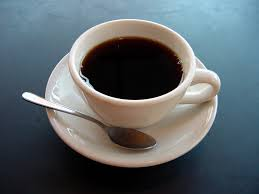
\includegraphics[width=\linewidth]{coffee.jpg}
     \caption{Coffee.}
  \end{subfigure}
  \begin{subfigure}[b]{0.2\linewidth}
    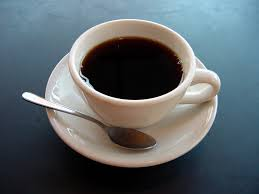
\includegraphics[width=\linewidth]{coffee.jpg}
    \caption{More coffee.}
  \end{subfigure}
  \begin{subfigure}[b]{0.2\linewidth}
    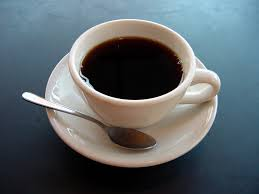
\includegraphics[width=\linewidth]{coffee.jpg}
    \caption{Tasty coffee.}
  \end{subfigure}
  \begin{subfigure}[b]{0.5\linewidth}
    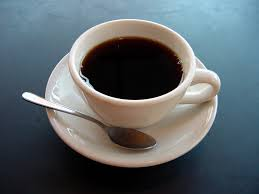
\includegraphics[width=\linewidth]{coffee.jpg}
    \caption{Too much coffee.}
  \end{subfigure}
  \caption{The same cup of coffee. Multiple times.}
  \label{fig:coffee3}
\end{figure}

\end{document}